\chapter{序論}
\label{chap_Introduction}

XXXXXXXXXXXXXXXXX序論

\section{先行研究}
現実的なハッシュテーブルを検討するには,
単にアルゴリズムのみならず,
対応する実実装との比較が望ましい.
ここでは,
実際に利用されているハッシュテーブルの実実装を示す.

\subsection{std::unorderd\_map}
C++ 標準のハッシュテーブル.
メモリ効率を重視しており速度は遅い.

\subsection{google::dense\_hash\_map}
最も探査の高速な実装の内の 1 つ.
スループットで 250 query/$\mu$s 程度
\footnote{AMD Ryzen7 1700 (8C/16T) 3.7 GHz の場合.詳細は,第\ref{chap_Results}章を参照.}
の探査速度を持つことから,
探査 1 回の実行時間は 4 ns
\footnote{
  $
    250{\rm [query \slash \mu s]}
    = \frac{1}{250} {\rm [\mu s \slash query]}
    = \frac{10^3}{250} {\rm [ns \slash query]}
    = 4 {\rm [ns \slash query]}
  $
}
である.このとき,3.7 GHz の CPU では単位 clock あたりの実行時間が,
$2.7 \times 10^{-1}$ [ns/clock]
\footnote{
  $
    \frac{1}{3.7 {\rm [GHz]}}
    = \frac{1}{3.7 \times 10^9}{\rm [sec]}
    = 2.7 \times 10^{-10}{\rm [sec]}
    = 2.7 \times 10^{-1}{\rm [ns/clock]}
  $
}
であるから,1 回の探査で消費する CPU cycle は
15 clock 程度
\footnote{
  $
    \frac{ 4 {\rm [ns/query]} }{ 2.7 \times 10^{-1} {\rm [ns/clock]} }
    = \frac{ 4 }{ 2.7 \times 10^{-1} } {\rm [clock/query]}
    \simeq 15 {\rm [clock/query]}
  $
}
である.

いくつかのハッシュテーブルでは,
key のハッシュ値をテーブルサイズに丸めるために剰余演算を用いる.
整数除算に必要な CPU cycle は 14--46 clocks 程度
\footnote{
  \cite{AgnerFog2018}より AMD Ryzen7 1700 の場合.
}
であるから,dense\_hash\_map の実行時間に対して計算量が大きい.
実際に,
dense\_hash\_map では,整数除算をしておらず,
ハッシュ値の LSB \footnote{Least Significant Bit の略記.最下位ビットのこと.} から
テーブルサイズ分の bit 数だけ bit mask 演算により取り出している.
これを実現するため,テーブルサイズは常に 2 のべき乗となるように制御されている.

また,メモリ使用量を削減するため,空マークを登録する必要があり,key として使用できない.

\subsection{ska::flat\_hash\_map}



%\begin{figure} % 特に強い理由がない限り、[htbp]のような指定はしないでください。
%  \centering
%  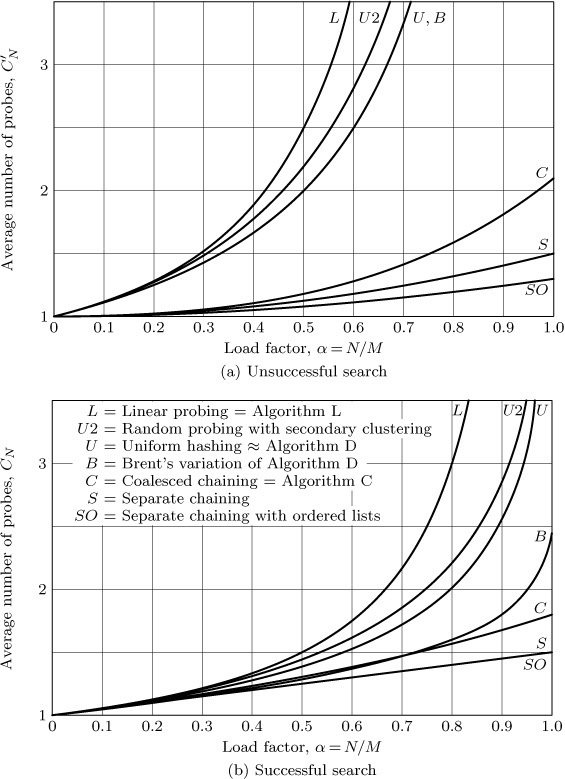
\includegraphics[width=10cm]{./figs/taocp_v3_fig44.png}
%  \caption{
%    Comparison of collision resolution methods: limiting values of the average number of probes as $M \rightarrow \infty$ \citep{knuth1998}.
%  }
%  \label{fig_taocp_v3_fig44}
%\end{figure}

%先行研究\footnote{脚注はこのように挿入します.}.


\section{Purpose}
研究目的.



















